\documentclass[a4paper, 11pt, twocolumn]{article}

\usepackage[utf8]{inputenc}

\usepackage[T1]{fontenc}

\usepackage[english]{babel}

\usepackage{graphicx}

 \usepackage{floatrow}

\usepackage[margin = 1in]{geometry}

\usepackage{float}

\usepackage[hidelinks]{hyperref}


\usepackage{url}

\usepackage{natbib}

%\usepackage[
%backend=biber,
%sorting=none
%]{biblatex}
\bibliographystyle{abbrvnat}
\setcitestyle{authoryear,open={(},close={)}}

\usepackage[most]{tcolorbox}

\usepackage{csquotes}

\usepackage{fancyhdr}


\usepackage{lipsum}

%\addbibresource{references.bib}

\title{\Large Internship report \\
\huge Alternative PCA algorithms analysis with missing values}


\author{Léopold Guyot}

\date{\today}

\begin{document}

\pagestyle{fancy}
\setlength{\headheight}{25.0117pt}
\fancyhead{}\fancyfoot{}
\fancyhead[L]{
\includegraphics[width = 0.2\textwidth]{img/LOGO_Universite__libre_bruxelles.png}}
\fancyhead[R]{Alternative PCA algorithms analysis with missing values}
\fancyfoot[R]{\thepage}

\onecolumn
\maketitle

\begin{tcolorbox}[breakable,colback=white,colframe=black,width=\dimexpr\textwidth+12mm\relax,enlarge left by=-6mm]

\section*{Abstract}


\end{tcolorbox}

\begin{figure}[H]
          \begin{minipage}{\textwidth}
                \centering
                
\includegraphics[width = .8\linewidth]{img/LOGO_Universite__libre_bruxelles.png}
          \end{minipage}
\end{figure}


\twocolumn
\section{Introduction}

Start with generic context
– Then zoom in: why is your approach necessary
and relevant within this context?
– Finish with a brief description of your method and
what you found out
– Read background information!
– Brief, 1 page (font size 11, normal margins)


- Presenting what is Single -Cell RNA seq.

- Explain why it is important to use SCRNAseq in some case

- Explain the dificulty of the modelisation part

- Present some models?

- Description on the content of the work

\section{Methods}
– Describe the datasets you are using
• Both their content and where you got them
– Describe the methods you implemented to get
your results
• Describe separate steps required (reproducibility!)
• Overview figures can help.
– 2-3 pages
\section{Results}

– Describe your results
• This can be in relation to:
– Different input/validation data
– Different method parameterisations, …
– Explain what the results mean
– Use tables for numbers (do not list in the text)
– Figures for distributions, relationships, … (easier
to understand than text)
– 2-3 pages
\begin{figure*}[!ht]
	\centering
	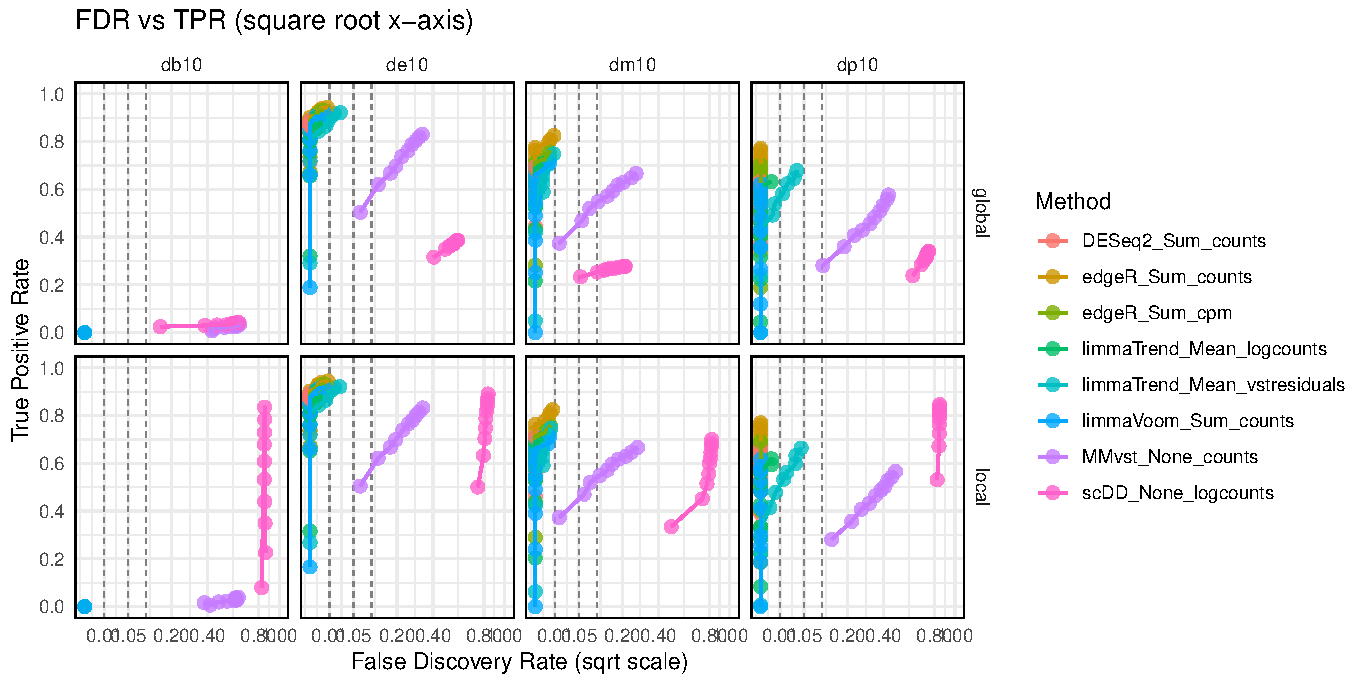
\includegraphics[width = \linewidth]{figs/fdrtpr_prop_method.pdf}
	\caption{
	}
	\label{fdrtpr_prop}
\end{figure*}

\begin{figure*}[!ht]
	\centering
	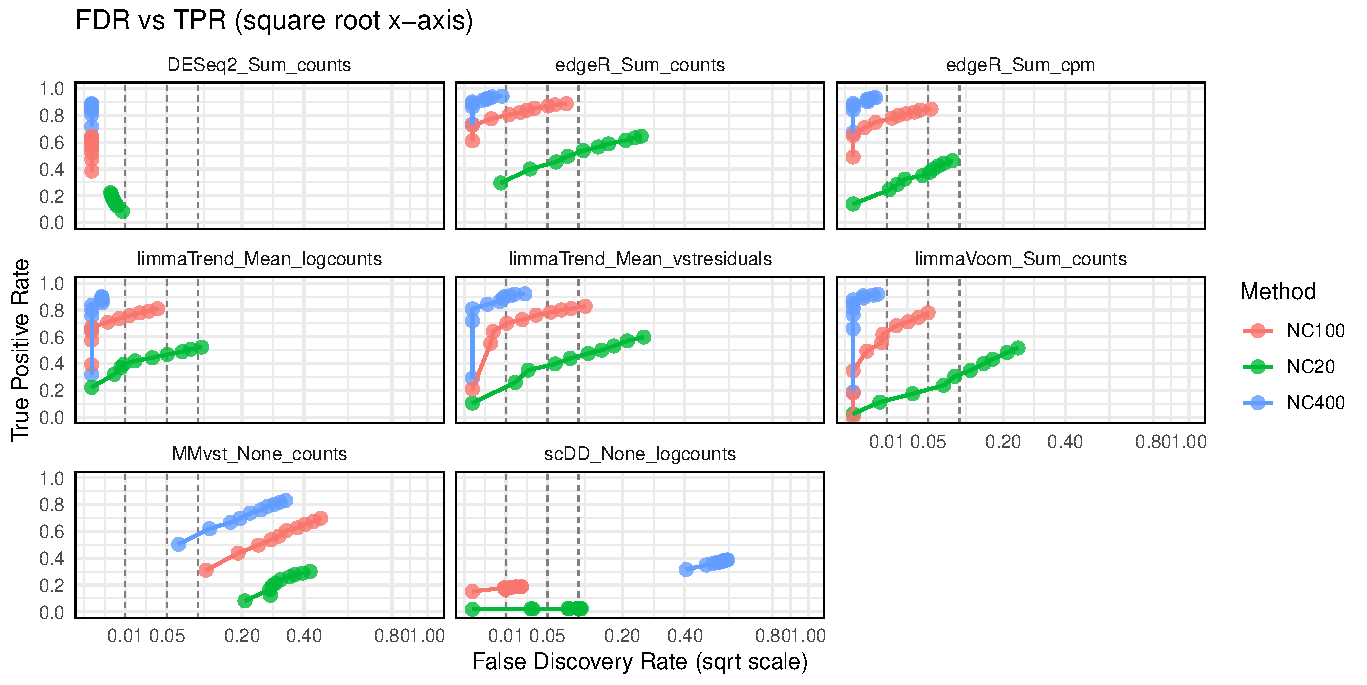
\includegraphics[width = \linewidth]{figs/fdrtpr_size_method.pdf}
	\caption{
	}
	\label{fdrtpr_size}
\end{figure*}

\section{Discussion}
Which issues did you identify, and which problems
did you encounter?
– What is different about your approach (and the
results you get) in comparison to the original
method? Why?
– What are advantages/disadvantage of each
method?
– 1 page
\section{Conclusion} 

\bibliography{references}

\end{document}
